\documentclass{article}
\usepackage{graphicx}
\usepackage{listings}
\usepackage{tikz}
\usetikzlibrary{positioning,fit,calc}
\tikzset{block/.style={draw,thick,text width=2cm,minimum height=1cm,align=center},
         line/.style={-latex}
}
\begin{document}

\title{CM30171}
\author{Rob Willison}

\maketitle
\tableofcontents

\section{Introduction}
This report is an explanation of the design decisions undertaked while writing
a --C compiler and interpreter.
\newpage
\section{Code Interpretation}

\section{Intermediate Code Generation}

\subsection{TAC Design}

The three address code used in the compiler was designed to be abstract enough as
too keep any machine dependent decisions out of the TAC stage. Many of the instructions
are obvious such as store and mathematic operations, examples below, and they won't be explained in
great detail.

\begin{lstlisting}
r2 := 1
r3 := r1 / r2
\end{lstlisting}

One thing to note about the store instruction is that in the event that the store
operand is defined in the scope above the current scope like x is in the following example.

\begin{lstlisting}
int main()
{
  int x = 4;
  int test()
  {
    return x;
  }

  return test();
}
\end{lstlisting}

In that scenario the store command in the test function will have an extra piece
of information saying that its defined in the scope one level above, so the store command will
look like the following.

\begin{lstlisting}
DEFINED IN 1 r2 := x
\end{lstlisting}

This information is also included when a closure is called from a narrower scope,
the TAC would be as follows.

\begin{lstlisting}
CALL _1 FROM SCOPE 1
\end{lstlisting}

For Functions a label instruction denotes the start and a end label for the end.
After the start label the new activation frame instruction which tells
the compiler to allocate space for a new activation frame with a given number
of arguments, locals and tempories. Before the end there is a return instruction
which contains the register with the value to return. Below is an example function
in TAC.

\begin{lstlisting}
_1:
NEW FRAME 0 arg 0 loc 1 temp
DEFINED IN 1 r2 := x
RETURN r2
FUNCTION END
\end{lstlisting}

There is one type of control sequence in the language, the if else, the way this
is described in TAC is using a sequence of if instructions and labels denoting the
various bodies if the if and else parts. An example in --C and the corresponding TAC
are below.

\begin{lstlisting}
if (1 > 4) {
  return 4;
} else if (2 > 1) {
  return 3;
}
\end{lstlisting}

\begin{lstlisting}
r1 := 1
r2 := 4
r3 := 1 > 4
IF NOT r3 GOTO 1
r4 := 4
RETURN 4
GOTO 2
LABEL 1: r5 := 2
r6 := 1
r7 := 2 > 1
IF NOT r7 GOTO 3
r8 := 3
RETURN 3
LABEL 3: LABEL 2:
\end{lstlisting}

Finally there is one loop type in the language, the while loop, this is translated
into a goto, an if and a label at the top and bottom of the loop body. the while
condition is placed after the body. n example in --C and the corresponding TAC
are below.

\begin{lstlisting}
int x = 0;
while (x < 5)
{
  x = x + 1;
}
\end{lstlisting}

\begin{lstlisting}
r1 := 0
x := r1
GOTO 1
LABEL 2: r2 := x
r3 := 1
r4 := r2 + r3
x := r4
LABEL 1: r5 := x
r6 := 5
r7 := r5 < r6
IF r7 GOTO 2
\end{lstlisting}

\subsection{TAC Generation}

All the TAC complilation is done in the tac\_compliler.c file.
In order to generate the TAC from source code a tree walk is performed over the
parse tree at each node depending on the type a set of TAC instructions are created
and added to the current TAC block. If a new function is found a new TAC block is
created before that part of the tree is parsed, also if a goto or label TAC instruction
are created new blocks are created. When a leaf is reached a store instruction is
created for the value at the leaf.\\~\\

\subsubsection{Enviroment Structure}

In order to keep track of the location of any local variables in the code and enviroment
is created to store the association between token and register location. The enviroment
is made up of frames each frame corresponds to a scope in the program and has
a linked list of all locals in that scope. The frames also contain a linked list of
the functions defined, these are a pair of token and label assigned to the function.
For example the environment created while walking the following piece of code is shown below.

\begin{lstlisting}
int main()
{
  int x = 4;
  int test()
  {
    int y = 5;
    return x * y;
  }

  return test();
}
\end{lstlisting}

\begin{tikzpicture}
  \node[block] (a) {Frame 1};
  \node[block,right=of a] (b) {Frame 2};
  \node[block] (c) at [yshift=-2cm] {x - r1};
  \node[block] (d) at [yshift=-4cm] {test - \_0};
  \node[block, right=of a] (e) at [yshift=-2cm, xshift=1.2cm] {y - r2};
  \draw[line] (a)-- (b);
  \draw[line] (a)-- (c);
  \draw[line] (c)-- (d);
  \draw[line] (b)-- (e);
\end{tikzpicture}

As you can see the environment holds the association between the tokens of the variables
and functions with the TAC register location and the function label respectively.

\subsubsection{TAC Blocking}

The diffrent blocks of TAC code, between labels and jumps, are separated to allow
easier optimisation and MIPS translation. As the AST is walked if a instruction which
requires a jump (If, While, Function Call) is found a new block is created and set as the
current block after the jump. Similarly if a label is created a new block is created
and the label is assigned to that new block.\\~\\
in order to compile the code in the same order as the TAC each block has a link to
the block which was created from the code directly after it. A Simple example is
given below.\\~\\

\begin{center}
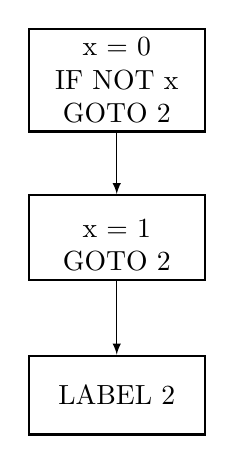
\begin{tikzpicture}
  \node[block] (a) {x = 0\\ IF NOT x GOTO 2};
  \node[block] [yshift=-2cm] (b) {\\ x = 1\\ GOTO 2};
  \node[block] [yshift=-4cm] (c) {LABEL 2};
  \draw[line] (a)-- (b);
  \draw[line] (b)-- (c);
\end{tikzpicture}
\end{center}

This was done so that the MIPS compilation step can easily follow the sequence of
TAC instructions. //TODO write about linking blocks if and when done

\subsubsection{Inner functions}

In order to implement inner functions, functions defined inside another, in TAC
the code for the function must be flattened so that there are no functions in functions
in the TAC. To do this when a function definition is reached inside another the current
TAC block is stored and another is created for the inner function, once the inner function's
AST has finished being walked the previous block is restored as the current block and
the AST tree walk continues. This gives the result of placing any inner functions after
the function it was defined in.

\subsection{TAC Optimisation}

After the TAC generation phase has been completed the sequence of blocks is handed
over to the optimisation phase. This is in the tac\_optimiser.c file. This applies
constant folding, copy propagation, dead code elimination, common sub expression
elimination and algebraic transformations algorithms to the TAC block repeatedly till
now change can be made. Each TAC block is processed from bottom to top for each
optimisation technique.

\subsubsection{Copy Propagation}

Copy propagation looks for a store instruction, once on is found it checks the
rest of the code below the store until it finds a write to the store destination.
For every read of the destination before replaced the use is replaced with the
stores operand. To demonstrate this copy propergation was applied to the same example
as above.

\begin{minipage}{0.3\textwidth}
\begin{lstlisting}

int x = 4;
int y = 6;

return x + y;

\end{lstlisting}
\end{minipage}%
\begin{minipage}{0.3\textwidth}
\begin{lstlisting}
r1 := 4
x := r1
r2 := 6
y := r2
r3 := x
r4 := y
r5 := r3 + r4
RETURN r5

\end{lstlisting}
\end{minipage}%
\begin{minipage}{0.3\textwidth}
\begin{lstlisting}
r1 := 4
x := 4
r2 := 6
y := 6
r3 := 4
r4 := 6
r5 := 4 + 6
RETURN r5
\end{lstlisting}
\end{minipage}%

\subsubsection{Constant Folding}

The constant folding function looks for arithmetic operations and replaces them
with the result where possible. This is done by looking for a operation where both
operands are tokens with type constant. Below is an example using both constant
folding and copy propergation.

\begin{minipage}{0.3\textwidth}
\begin{lstlisting}

int x = 4;
int y = 6;

return x + y;

\end{lstlisting}
\end{minipage}%
\begin{minipage}{0.3\textwidth}
\begin{lstlisting}
r1 := 4
x := 4
r2 := 6
y := 6
r3 := 4
r4 := 6
r5 := 4 + 6
RETURN r5

\end{lstlisting}
\end{minipage}%
\begin{minipage}{0.3\textwidth}
\begin{lstlisting}
r1 := 4
x := 4
r2 := 6
y := 6
r3 := 4
r4 := 6
r5 := 10
RETURN 10
\end{lstlisting}
\end{minipage}%

\subsubsection{Dead Code Elimination}

Dead code elimination works by analysing each instruction using and useing the
next use info removes them if not needed. Firstly this is only done for registers
user defined variables are live at the end of the block so an't removed. A instruction
is removed if the next use is not live, its another write, or there isn't another
next use. Using the same example as above and applying dead code elimination gives
the following.

\begin{minipage}{0.3\textwidth}
\begin{lstlisting}

int x = 4;
int y = 6;

return x + y;

\end{lstlisting}
\end{minipage}%
\begin{minipage}{0.3\textwidth}
\begin{lstlisting}
r1 := 4
x := 4
r2 := 6
y := 6
r3 := 4
r4 := 6
r5 := 10
RETURN 10

\end{lstlisting}
\end{minipage}%
\begin{minipage}{0.3\textwidth}
\begin{lstlisting}
RETURN 10
\end{lstlisting}
\end{minipage}%

\subsubsection{Common Sub Expression Elimination}
If two expression have the same operands and operation the later one can be replaced
with a store of the destination of the first. These are found by looking for pairs
of arithmatic operations, when one is found if the operation and operands are the
same the second is replaced with a store. An exaple is given below usign this method
in conjunction with copy propergation.

\begin{minipage}{0.3\textwidth}
\begin{lstlisting}

int c = 4 * 6;
int d = 4 * 6;

return c;

\end{lstlisting}
\end{minipage}%
\begin{minipage}{0.3\textwidth}
\begin{lstlisting}
r1 := 4
r2 := 6
r3 := r1 * r2
c := r3
r4 := 4
r5 := 6
r6 := r4 * r5
d := r6
r7 := c
RETURN r7
\end{lstlisting}
\end{minipage}%
\begin{minipage}{0.3\textwidth}
\begin{lstlisting}
r1 := 4
r2 := 6
r3 := 4 * 6
c := r3
r4 := 4
r5 := 6
r6 := r3
d := r3
r7 := r3
RETURN r3
\end{lstlisting}
\end{minipage}%

\subsubsection{Algebraic Transformations}

The final optimisation technique is to transform some algebraic expressions
which will always give 1 or 0 to those values. In order to do this the optimiser
looks for those specific expressions and simply replaces them with a store of either
1 or 0 depending on the expression. An example is given below using copy propagation
aswell.

\begin{minipage}{0.3\textwidth}
\begin{lstlisting}

int x = test();
int a = 0 + x;

return a;
\end{lstlisting}
\end{minipage}%
\begin{minipage}{0.3\textwidth}
\begin{lstlisting}
CALL _1
r2 := result
x := result
r3 := 0
r4 := result
r5 := 0 + result
a := r5
r6 := r5
RETURN r5
\end{lstlisting}
\end{minipage}%
\begin{minipage}{0.3\textwidth}
\begin{lstlisting}
CALL _1
r2 := result
x := result
r3 := 0
r4 := result
r5 := result
a := result
r6 := result
RETURN result
\end{lstlisting}
\end{minipage}%



\section{Machine Code Generation}

\end{document}